\section{Introduzione: Gradle} % https://github.com/gradle/gradle 
Gradle è un progetto open source che fornisce un tool di build automation, che può essere un ottimo sostituto di Maven. Offre un modello in grado di sostenere l'intero ciclo di vita dello sviluppo del software ed è stato progettato per supportare build automation attraverso più linguaggi e piattaforme. Nel nostro caso considereremo questo tool per lo sviluppo di software Java.

\subsection{Differenze tra Gradle e Maven}
Uno dei build tool più usati attualmente è senza dubbio Maven. Ci sono molte differenze tra questi due tools: flessibilità, performance, gestione delle dipendenze e molto altro. Le differenze si possono già notare dal file di configurazione, Gradle infatti ha una convenzione molto più facile e comprensibile rispetto alla tediosa configurazione del pom di Maven. Anche se entrambi usano dei metodi di miglioramento della velocità di esecuzione delle build, Gradle è senza dubbio il tool più veloce. Per essere migliore Grandle usufruisce di:
\begin{itemize}
    \item \textbf{Incrementality:} evitando il lavoro di monitoraggio dei task di I/O eseguendo solo il necessario e quando possibile processare solo i files che sono cambiati;
    \item \textbf{Build Cache:} utilizza un sistema di cache riusando gli outputs di altre build Gradle con gli stessi inputs;
    \item \textbf{Deamon:} sfrutta un long-lived process che mantiene tutte le informazioni in memoria.
\end{itemize}
Queste 3 caratteristiche rendono Gradle molto veloce, ad esempio una build Gradle con Maven verrebbe completata con un tempo 3 volte maggiore. Tutto questo è anche possibile grazie a un sistema di esecuzioni parallele di task e intra-task.
\begin{figure}[H]
\centering
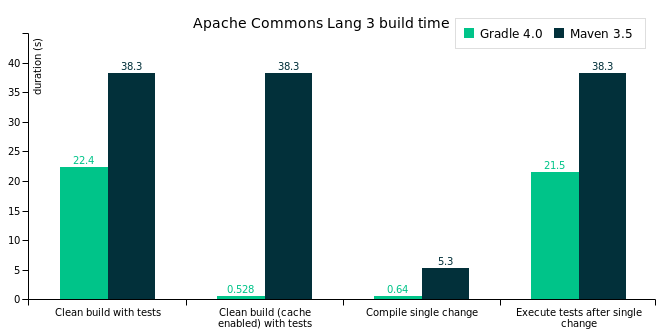
\includegraphics[width=0.7\linewidth]{0introduction/gradle/performance.png}
\end{figure}
Possiamo quindi affermare che Gradle può essere un ottimo sostituto di Maven.

(La relazione è stata scritta per SO Linux, ma i concetti generali valgono per tutti)
\subsection{Installazione}
L'istallazione di Gradle può essere fatta in più modi: tramite installazione manuale o utilizzando un package manager (tutte le informazioni possono essere trovate in \textbf{\href{https://gradle.org/install/}{questo link}}). Personalmente consiglio l'utilizzo del software development kit manager \textbf{\href{http://sdkman.io/}{SDKMAN!}} che non solo permette l'installazione molto facilitata di Gradle, ma anche della JVM e di tanti altri tools. L'installazione si basa su 2 semplici comandi:
\begin{verbatim}
  $ curl -s "https://get.sdkman.io" | bash
  
  $ source "$HOME/.sdkman/bin/sdkman-init.sh" \end{verbatim}
A questo punto se tutto è andato a buon fine SDKMAN! è stato installato correttamente, è possibile verificarlo digitando il comando su terminale:
\begin{verbatim}
  $ sdk version \end{verbatim}
l'output risultante dovrebbe essere qualcosa del tipo:
\begin{verbatim}
  SDKMAN 5.5.15+284 \end{verbatim}
Ora è possibile procedere con l'installazione di Gradle. Prima di tutto visualizziamo la lista delle versioni di Gradle:
\begin{verbatim}
  $ sdk list gradle \end{verbatim}
L'output corrispondente sarà:
\begin{verbatim}
================================================================================
Available Gradle Versions
================================================================================
     4.6-rc-2             4.3.1                3.5                  2.2.1          
     4.6-rc-1             4.3-rc-4             3.4.1                2.2            
     4.6                  4.3-rc-3             3.4                  2.14.1         
     4.5.1                4.3-rc-2             3.3                  2.14           
     4.5-rc-2             4.3-rc-1             3.2.1                2.13           
     4.5-rc-1             4.3                  3.2                  2.12           
     4.5                  4.2.1                3.1                  2.11           
     4.4.1                4.2-rc-2             3.0                  2.10           
     4.4-rc-6             4.2-rc-1             2.9                  2.1            
     4.4-rc-5             4.2                  2.8                  2.0            
     4.4-rc-4             4.1                  2.7                  1.9            
     4.4-rc-3             4.0.2                2.6                  1.8            
     4.4-rc-2             4.0.1                2.5                  1.7            
     4.4-rc-1             4.0                  2.4                  1.6            
     4.4                  3.5.1                2.3                  1.5            

================================================================================
+ - local version
* - installed
> - currently in use
================================================================================ \end{verbatim}
La versione che vogliamo installare è quella più recente che in questo caso è la 4.6, possiamo quindi eseguire il comando:
\begin{verbatim}
  $ sdk install gradle 4.6 \end{verbatim}
appena il download e l'installazione sarà finita possiamo verificare il completamento tramite:
\begin{verbatim}
  $ gradle -v \end{verbatim}
che non solo stamperà su terminale la versione di Gradle, ma anche:
\begin{itemize}
  \item \href{http://www.groovy-lang.org/}{Groovy} (linguaggio di programmazione usato per scrivere i file di configurazione)
  \item Ant (software usato per le build delle Java applications)
  \item Java Virtual Machine
  \item sistema operativo in uso
\end{itemize}
se l'output ha queste informazioni allora Gradle è stato completamente installato. SDKMAN! si preoccupa anche di creare la variabile \$GRADLE\_HOME che è possibile visualizzare con il comando 
\begin{verbatim} 
    $ echo $GRADLE_HOME \end{verbatim} 
Se ci sono errori di tipo Java, i problemi possono essere:
\begin{itemize}
  \item Gradle non riesce a trovare la jdk, problema risolvibile installando java con sdkman con il comando 
  \begin{verbatim}
    $ sdk install java <versione>  \end{verbatim}
  \item Java è aggiornato alla versione 9 o superiori (infatti attualmente Gradle non è aggiornato per versioni superiori alla 8), basterà fare un downgrade ad una versione precedente (possibile farlo anche tramite SDKMAN!).
\end{itemize}
In entrambi i casi sarà necessario anche comunicare al sistema la versione da usare: 
\begin{verbatim}  
    $ sdk dafault java <versione_installata> \end{verbatim} 
per essere sicuri che è stata installata la giusta versione di java possiamo controllare gli outputs dei seguenti comandi:
\begin{itemize}
  \item \begin{verbatim} $ echo $JAVA_HOME \end{verbatim}
  \item \begin{verbatim} $ java -version \end{verbatim}
\end{itemize}
il primo comando dovrà restituire in output il giusto percorso della JVM installata, il secondo serve a controllare la versione java attualmente in uso.

